%
%
%
\section{Plane waves and unit cells}

A plane wave is a type of wave in which the wavefronts (surfaces of constant phase) are infinitely large, flat planes. The wave travels in a uniform direction, and at any given moment, the wave's amplitude and phase are constant across any plane perpendicular to the direction of propagation. 

A unit cell is the smallest, repeating structural unit of a (crystal) lattice that, when stacked in three-dimensional space, forms the entire (infinite) structure. It represents the basic building block of the lattice and contains the arrangement of atoms that are repeated throughout the material to create the full structure.

In plane wave density functional theory, plane waves are used to describe the electronic structure of a system in the sense that they are used as basis functions. In contrast to localized-orbital density functional theory, plane waves are not associated to a specific atom, but should be thought of as spawned by the unit cell in which the atoms reside.

In the following, I will provide a mathematical framework to describe both plane waves and unit cells and how the two are related within the context of this work.

%
%
%
\subsection{Mathematical framework}

Consider a periodic unitcell defined by the matrix $\mathbf{M}$ which encapsulates the triplet of vectors spanning the parallelepiped in its row-space as given by

\begin{equation}
    \mathbf{M} = \left(
    \begin{matrix}
        \vec{a_{1}}\\
        \vec{a_{2}}\\
        \vec{a_{3}}
    \end{matrix}
    \right).
\end{equation}

A schematic representation is provided in \cref{fig:unitcell}.

\begin{Figure}
    \centering
    \resizebox{0.7 \textwidth}{!}{
        \begin{tikzpicture}

% Draw cube
\draw[dashed, color=gray] (0,0,0) -- (3,0,0) -- (3,3,0) -- (0,3,0) -- cycle; % front face
\draw[dashed, color=gray] (0,0,3) -- (3,0,3) -- (3,3,3) -- (0,3,3) -- cycle; % back face
\draw[dashed, color=gray] (0,0,0) -- (0,0,3); % connecting lines
\draw[dashed, color=gray] (3,0,0) -- (3,0,3);
\draw[dashed, color=gray] (3,3,0) -- (3,3,3);
\draw[dashed, color=gray] (0,3,0) -- (0,3,3);

% Label axes
\draw[thick,->] (0,0,0) -- (3,0,0) node[anchor=west] {$\vec{a}_{2}$}; 
\draw[thick,->] (0,0,0) -- (0,3,0) node[anchor=south] {$\vec{a}_{3}$}; 
\draw[thick,->] (0,0,0) -- (0,0,3) node[anchor=north east] {$\vec{a}_{1}$}; 

\end{tikzpicture}
    }
    \captionof{figure}{Schematic depiction of a (cubic) unit cell spanned by the triplet of vectors $\{\vec{a}_{1}, \vec{a}_{1}, \vec{a}_{1}\}$.}
    \label{fig:unitcell}
\end{Figure}

The volume of this unit cell ($\Omega$) is given by the absolute value of the determinant of $\mathbf{M}$ or similarly by the triple product of its unit vectors.

\begin{equation}
    \Omega = \det \left| \mathbf{M} \right| = \vec{a_{1}} \cdot \left(\vec{a_{2}} \times \vec{a_{3}} \right)
\end{equation}

Any point $\vec{r}$ within this unit cell is equivalent to another point 

\begin{equation}
    \vec{r} = \vec{r} + \vec{R}
\end{equation}

wherein

\begin{equation}
    \vec{R} = n_{1}\vec{a_{1}} + n_{2}\vec{a_{2}} + n_{3}\vec{a_{3}} \; \text{with} \; n_{1},n_{2},n_{3} \in \mathbb{Z}.
\end{equation}

For an arbitrary unitcell $\mathbf{M}$, we can define a set of plane waves $\{ \phi(\vec{G},\vec{r}) \}$ wherein each plane wave is given by

\begin{equation}
    \phi(\vec{G},\vec{r}) = \frac{1}{\sqrt{\Omega}} \exp \left(i \vec{G} \cdot \vec{r} \right),
    \label{eq:pwexpr}
\end{equation}

wherein $i = \sqrt{-1}$ is the imaginary number and $\vec{G}$ a plane wave vector corresponding to

\begin{align}
    \vec{G}_{i_{1},i_{2},i_{3}} = 
    &\left(i_{1} - \frac{N_{1}}{2} \right)\vec{b_{1}} + \label{eq:gvectors} \\ \nonumber
    &\left(i_{2} - \frac{N_{2}}{2} \right)\vec{b_{2}} + \\ \nonumber
    &\left(i_{3} - \frac{N_{3}}{2} \right)\vec{b_{3}}
\end{align}

which in turn are derived from the reciprocal lattice vectors $\vec{b}_{i}$ which are given by

\begin{align}
    \vec{b_{1}} &= 2 \pi \frac{\vec{a_{2}} \times \vec{a_{3}}}{\Omega} \label{eq:reciproc-latv1} \\ 
    \vec{b_{2}} &= 2 \pi \frac{\vec{a_{3}} \times \vec{a_{1}}}{\Omega} \label{eq:reciproc-latv2} \\ 
    \vec{b_{3}} &= 2 \pi \frac{\vec{a_{1}} \times \vec{a_{2}}}{\Omega} \label{eq:reciproc-latv3}
\end{align}

where $N_{1}$, $N_{2}$, $N_{3}$ act as the number of discretization points used to sample the real-space unitcell and $0 \leq i_{x} < N_{x}$ with $x \in 1,2,3$.

Alternatively, the matrix $\mat{B}$ describing the reciprocal lattice vectors in its row space can be obtained via

\begin{equation}
    \mat{B} = \left(
    \begin{matrix}
        \vec{b_{1}}\\
        \vec{b_{2}}\\
        \vec{b_{3}}
    \end{matrix}
    \right) = 2 \pi \left( \mat{M}^{\intercal} \right)^{-1},
\end{equation}

where $M^{\intercal}$ indicates the matrix transpose of $\mat{M}$.

To illustrate the above, consider a cubic unitcell, which can be represented by the matrix $\mathbf{M}$ according to

\begin{equation}
    \mathbf{M} = a \mathbf{I}_{3},
\end{equation}

$\mathbf{I}_{3}$ being the 3x3 identity matrix and $a$ the lattice constant, the reciprocal lattice vectors $\{\vec{b}_{i}\}$ correspond to

\begin{align}
    \vec{b}_{1} &= \frac{2\pi}{a} \left(1,0,0\right) \\
    \vec{b}_{2} &= \frac{2\pi}{a} \left(0,1,0\right) \\
    \vec{b}_{3} &= \frac{2\pi}{a} \left(0,0,1\right).
\end{align}

%
%
%
\subsection{Orthonormality relationship}

The plane waves spanned from a single unit cell form an orthonormal set. The orthonormality relationship can be readily verified by evaluating the following expression

\begin{align}
    \braket{\phi(\vec{G},\vec{r}) | \phi(\vec{G},\vec{r})} &= \frac{1}{\Omega} \int_{\Omega} d \vec{r} \;\exp \left(-i \vec{G} \cdot \vec{r} \right) \exp \left(+i \vec{G} \cdot \vec{r} \right) \\
    &= \frac{1}{\Omega} \int_{\Omega} d \vec{r} \; 1 = \frac{\Omega}{\Omega} = 1. \\
\end{align}

In the above equation, observe that the complex conjugate is taken for the function $\phi(\vec{G},\vec{r})$ when used in the \textit{bra}, as required by the rules for an inner product in Hilbert space.\footnote{I have also pedantically introduced a ``+'' for the \textit{ket} part just to emphasize on this aspect.} Generalizing the above expression for any two plane waves, including those with different $\vec{G}$-vectors, we find that

\begin{align}
    \braket{\phi(\vec{G}\prime,\vec{r}) | \phi(\vec{G},\vec{r})} &= \frac{1}{\Omega} \int_{\Omega} d \vec{r} \; \exp\left(-i \vec{G}\prime \cdot \vec{r} \right) \exp\left(+i \vec{G} \cdot \vec{r} \right) \\
    &= \frac{1}{\Omega} \int_{\Omega} d \vec{r} \; \exp\left(i \left(\vec{G} - \vec{G}\prime \right) \cdot \vec{r} \right) \\
    &= \delta_{\vec{G},\vec{G}\prime} \label{eq:pw-ortho}
\end{align}

where $\delta_{\vec{G},\vec{G}\prime}$ represents the Kronecker delta function which is defined such that

\begin{equation}
    \delta_{\vec{G},\vec{G}\prime} =
    \begin{cases}
    1\; \text{if}\; \vec{G} = \vec{G}\prime \\
    0\; \text{otherwise}
    \end{cases}
\end{equation}

From the result of \cref{eq:pw-ortho} it can thus be concluded that two plane waves, whose wave vectors $\vec{G}$ obey \cref{eq:gvectors}, that have difference values for $\vec{G}$ are orthogonal functions with respect to each other.

%
%
%
\subsection{Evaluation of expansion coefficients}

Any arbitrary function $u(\vec{r})$ that resides inside the unit cell that meets the condition

\begin{equation}
    u(\vec{r}) = u(\vec{r} + \vec{R}) \label{eq:perfunc}
\end{equation}

can be represented by a plane wave expansion in the sense that

\begin{equation}
    u(\vec{r}) = \frac{1}{\sqrt{\Omega}} \sum_{\vec{G}} \tilde{u}(\vec{G}) \exp \left(i \vec{G} \cdot \vec{r} \right), \label{eq:plane-wave-exp}
\end{equation}

where $\tilde{u}(\vec{G}) \in \mathbb{C}$ act as the plane wave expansion coefficients. In the above expansion, the plane waves $\phi(\vec{G},\vec{r})$ thus act as \textbf{basis functions} and the complete set of plane waves $\left\{ \phi(\vec{G},\vec{r}) \right\}$ is termed the \textbf{plane wave basis set}.

To find the plane wave expansion coefficients $\tilde{u}(\vec{G})$, consider the integral $\braket{\phi(\vec{G}\prime,\vec{r}) | u(\vec{r})}$, which by application of \cref{eq:pw-ortho,eq:plane-wave-exp} yields

\begin{align}
    \braket{\phi(\vec{G}\prime,\vec{r}) | u(\vec{r})} &= \int_{\Omega} d\vec{r} \; \frac{1}{\Omega} \sum_{\vec{G}} \tilde{u}(\vec{G}) \exp \left(i \left(\vec{G} - \vec{G}\prime\right) \cdot \vec{r} \right) \label{eq:pwcoeff-int} \\
    &= \sum_{\vec{G}} \tilde{u}(\vec{G}) \delta_{\vec{G},\vec{G}\prime} \\
    &= \tilde{u}(\vec{G}\prime).
\end{align}

As can be seen, the above integral provides a mathematical recipe for finding the plane wave expansion coefficients $\tilde{u}(\vec{G})$ for any vector $\vec{G}$, exploiting the orthonormality relationship among the plane waves.

%
%
%
\subsection{Basis set truncation}

With the aim to actually use a plane wave expansion to describe an arbitrary function, it becomes relevant to more accurately define the basis set. Fundamentally speaking, the number of discretization points ($N_{1}$, $N_{2}$ and $N_{3}$) in \cref{eq:gvectors} can be chosen arbitrarily large, yet from a computational point of view it makes sense to truncate the expansion of \cref{eq:plane-wave-exp} by allowing only those plane waves whose kinetic energy is less than a certain threshold value. This threshold value is termed the cut-off energy. The kinetic energy of a plane wave is found via

\begin{align}
    E_{k} &= \left<\phi(\vec{G},\vec{r}) \left| -\frac{1}{2} \nabla^{2} \right|\phi(\vec{G},\vec{r})\right> \\
    &= \frac{1}{2} \left| \vec{G} \right|^{2}
    \label{eq:kin-en_pw}
\end{align}

and corresponds to half the squared modulus of the plane wave vector $\vec{G}$. The set of plane waves characterized by a cut-off energy $E_{\textrm{cut}}$ are those plane waves which obey

\begin{equation}
    \frac{1}{2} \left| \vec{G} \right|^{2} < E_{\textrm{cut}}.
\end{equation}

%
%
%
\subsection{Fast Fourier transforms}

Although \cref{eq:pwcoeff-int} provides a straightforward recipe to find the $\tilde{u}(\vec{G})$, when one is tasked to find the set $\{\tilde{u}(\vec{G})\}$ it turns out that there is a significantly more efficient numerical recipes available, known as the Fast Fourier transform (FFT). Uniquely, the FFT tactically exploits common operations in the evaluation of the integrals for plane waves within the same set (e.g. those spanned from the same unit cell) such that in contrast to the typical $N^{3}$ scaling observed in numerical integration, one obtains a mere $N \log N$ scaling. As both algorithms are able to make efficient use of multi-core computational architectures, the scaling relationship is the dominant discriminating factor between the two procedures. As such, it should be clear from the scaling relationship that usage of FFT algorithms to calculate the expansion coefficient evaluations are the preferred choice.

The FFT algorithm is provided in many software packages for a diverse array of programming languages and environments. Just for the Python programming language alone, there are already three commonly-used libraries available, corresponding to those implemented in NumPy\cite{numpy} and SciPy\cite{scipy} and one dedicated module PyFFTW. These libraries differ in their ease of use and computational efficiency, yet all perform the FFT using the same underlying mathematical conventions and thus yield the same result. It is relevant to emphasize here that this does not have to be the case and before using any kind of numerical implementation of the FFT, one should critically read its documentation to assess which conventions are in place.

The way that the FFT works is that it takes as input a discretized scalar field, i.e. the values of the function $f_{i} = f(\vec{r_{i}})$ taken at sampling points $\left\{\vec{r}_{i}\right\}$. The output of the FFT corresponds to the values of the expansion coefficients $\tilde{f}(\vec{G_{i}})$ for the set of plane wave vectors $\left\{ \vec{G}_{i} \right\}$. The sets $\left\{\vec{r}_{i}\right\}$ and $\left\{\vec{G}_{i}\right\}$ are related in the sense that they both pertain to an equidistant discretization of their corresponding spaces, i.e. \textbf{real-space} and \textbf{reciprocal-space} representations, and are of the same size and dimensionality. The FFT thus acts as a basis set transformation between basis functions spanning the real-space and another basis set spanning the reciprocal-space, the latter set being the plane waves.

\begin{Figure}
    \centering
    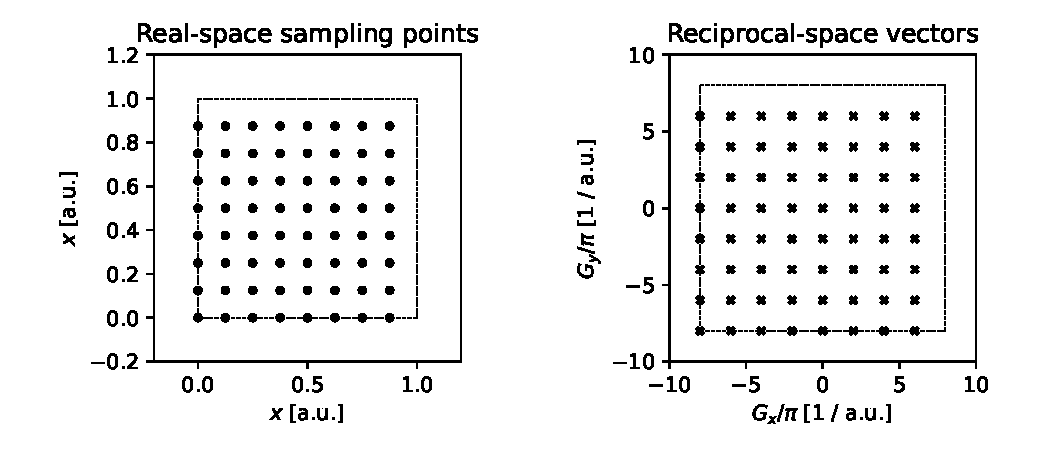
\includegraphics[width=\linewidth]{img/sampling.pdf}
    \captionof{figure}{Schematic depiction of (left) sampling points in real-space for a cubic unit cell of $1 \times 1 \times 1$ a.u. and (right) the corresponding plane-wave vectors in reciprocal-space. The real-space sampling points are shown for $z=0.5$ and the reciprocal lattice vectors are shown for $G_{z}=0$. The dashed lines indicate the real (left) and reciprocal (right) unit cells.}
    \label{fig:sampling}
\end{Figure}

In \cref{fig:sampling}, an example is provided for a cubic unit cell with edges of size $a_{0} = 1$ a.u. and $N = 8$ sampling points per Cartesian direction. In the graph on the left hand side, we can see the 64 sampling points that lie in the plane $z=5$. In total, there are 8 such planes in which the values for the function to be transformed are going to be sampled. Application of the FFT will result in the expansion coefficients for the set of plane waves whose reciprocal lattice vectors are shown in the right graph in \cref{fig:sampling}. Observe that with increasing distance from the origin, the $\vec{G}$-vectors corresponds to increasingly stronger oscillating plane waves with increasing kinetic energy.

Since the plane waves are periodic functions, there is some level of arbitrariness to the exact position of the sampling points. We are allowed to translate all sampling points by a displacement vector $\vec{d}$ as long as the periodicity of the unit cell is respected. Slightly different expansion coefficients can perhaps be obtained, but when a sufficiently dense sampling grid is taken, numerical differences are expected to be minimal.

The FFT implementation in NumPy, Scipy and PyFFTW is defined such that the value at $f(\vec{r_{i}})$ is calculated from the expansion coefficients $\tilde{f}(\vec{G_{i}})$ via

\begin{equation}
    f(\vec{r}_{i}) = \frac{1}{N_{x}N_{y}N_{z}} \sum_{\vec{G}} \tilde{f}(\vec{G}) \exp \left(i \vec{G} \cdot \vec{r}_{i} \right).
\end{equation}

This definition however differs from the one used in \cref{eq:plane-wave-exp}, though only by a multiplicative factor

\begin{equation}
    C_{t} = \frac{\sqrt{\Omega}}{N_{x}N_{y}N_{z}}.
    \label{eq:ct}
\end{equation}

This means that we can readily use the output of the FFT as implemented in these libraries and perform a simple scalar multiplication

\begin{align}
    \left\{\tilde{u}(\vec{G})\right\} &= C_{t} \cdot \fft\left[\left\{ u(\vec{r}) \right\}\right] \\
    &= \fftpw\left[\left\{ u(\vec{r}) \right\}\right]
\end{align}

to obtain the expansion coefficients complying with \cref{eq:plane-wave-exp}. Throughout this work, we will therefore diferentiate between the FFT transform as provided by the computational library, indicated by $\fft$ and the FFT transform needed to comply with our plane wave basis set, indicated by $\fft_{\text{pw}}$.

Complementary to the FFT from real-space to reciprocal-space, there is also the reverse or inverse operation, indicated by $\ifft$ and $\ifftpw$.

\begin{align}
    \left\{ u(\vec{r}) \right\} &= \frac{1}{C_{t}} \ifft\left[\left\{\tilde{u}(\vec{G})\right\}\right] \\
    &= \ifftpw\left[\left\{\tilde{u}(\vec{G})\right\}\right]
    \label{eq:fft_pw_inverse}
\end{align}

By its very definition, it thus follows that sequential application of the FFT and its inverse (or \textit{vice versa} corresponds to performing an identity operation, i.e.

\begin{equation}
    f(\vec{r}) = \ifft\left[\fft\left[f(\vec{r})\right]\right]
\end{equation}

%
%
%
\subsubsection{Properties of FFTs}

FFT have a number of relevant properties. Here, I will mention those that are relevant to our endeavour to use them in a density functional theory code.

\begin{itemize}
    \item 

    The FFT is a linear transformation in the sense that

    \begin{equation}
        \fft\left[a f(\vec{r}) + bg(\vec{r}) \right] = a\tilde{f}(\vec{G}) + b\tilde{g}(\vec{G}).
    \end{equation}
    
    Thus, the FFT of a sum of functions yields the sum of the FFTs. Furthermore, any multiplicative constant is simply forwarded in the transform.

    \item 

    A convolution in real-space corresponds to a product in reciprocal-space and likewise, a product in real-space is a convolution in reciprocal-space. Thus,

    \begin{equation}
        \fft\left[f(\vec{r}) \ast g(\vec{r}) \right] = \tilde{f}(\vec{G}) \cdot \tilde{g}(\vec{G})
    \end{equation}

    and

    \begin{equation}
        \ifft\left[\tilde{f}(\vec{G}) \ast \tilde{g}(\vec{G}) \right] = f(\vec{r}) \cdot g(\vec{r}).
    \end{equation}

    The implication of this property is that certain operations are best executed in real-space or in reciprocal-space. A salient example is the evaluation of the electron density. Since this corresponds to the product of the wave function with itself, this is best executed in real-space. In contrast, the evaluation of the classical electrostatic energy of a charge cloud corresponds to a convolution in real-space and is thus most effectively evaluated in reciprocal-space where it only constitutes a product.

    \item

    The FFT of a real-valued scalar field produces a symmetric transform. This can be readily understood from the fact that sampling with a plane wave that osscillates in the positive direction yields in principle the same result as one that oscillates in the negative direction, though with its imaginary part inverted. Thus, for a transform
    
    \begin{equation}
        \tilde{f}(\vec{G}) = \fft\left[f(\vec{r})\right],\;\text{with}\;f(\vec{r}) \in \mathbb{R}^{3}
    \end{equation}
    
    we find that
    
    \begin{equation}
        \tilde{f}(\vec{G}) = \tilde{f}(-\vec{G})^{*},
    \end{equation}

    where $^{*}$ indicates the complex conjugate.
    
\end{itemize}

The relevance and implications of these properties will be further clarified in the following text. If the reader has not yet fully grasped their significance, the remaining sections in this document should provide better context and understanding.

%
%
%
\subsubsection{Sampling of properties using plane waves}

Certain properties are more effectively sampled in real-space, while others are better suited to reciprocal-space. Here, we demonstrate how kinetic energy can be evaluated using a plane wave basis set, taking advantage of the orthonormality property of this set. Kinetic energy, in particular, is a property that can be almost effortlessly sampled in reciprocal-space. To illustrate this, consider the wave function $\psi(\vec{r})$ as expanded in plane waves via

\begin{align}
    \psi(\vec{r}) &= \frac{1}{\sqrt{\Omega}} \sum_{\vec{G}} \tilde{\psi}(\vec{G}) \exp \left(i \vec{G} \cdot \vec{r} \right) \\
    &= \sum_{\vec{G}} \tilde{\psi}(\vec{G}) \phi(\vec{G}).
\end{align}

Building upon the derivation of the kinetic energy of a single plane wave as shown in \cref{eq:kin-en_pw}, we can readily show that for $\psi(\vec{r})$ we find

\begin{align}
    E_{\text{kin}} &= \left<\psi(\vec{r})\left|-\frac{1}{2}\nabla^{2}\right|\psi(\vec{r})\right> \\
    &= \frac{1}{2} \sum_{\vec{G}\prime}\sum_{\vec{G}} \tilde{\psi}(\vec{G}) \tilde{\psi}(\vec{G}\prime) |\vec{G}|^{2} \braket{\phi(\vec{G}\prime)|\phi(\vec{G})} \\
    &= \frac{1}{2} \sum_{\vec{G}\prime}\sum_{\vec{G}} \tilde{\psi}(\vec{G}) \tilde{\psi}(\vec{G}\prime) |\vec{G}|^{2} \delta_{G,G\prime} \\
    &=\frac{1}{2}\sum_{\vec{G}} |\tilde{\psi}(\vec{G})|^{2} \cdot |\vec{G}|^{2}
\end{align}

wherein $\phi(\vec{G})$ corresponds to a single plane wave in line with \cref{eq:pwexpr}.

%
%
%
\subsubsection{Demonstration for the 1s orbital of H}

To tie everything together in this section, let us provide a detailed example for the $1s$ atomic orbital of H. Consider a hydrogen atom at position $\vec{R}$ located inside a unitcell with dimensions of $10 \times 10 \times 10$ a.u. The wave function corresponding to the $1s$ atomic orbital, in atomic units, is given by

\begin{equation}
    \psi_{\text{1s}} = \frac{1}{\sqrt{\pi}} \exp \left( -|\vec{r} - \vec{R}| \right),
    \label{eq:horb_1s}
\end{equation}

where $\vec{R} = (5,5,5)$.

To produce the FFT, the function $\psi_{\text{1s}}$ is sampled on the interval $x,y,z \in (0,10)$, using 64 sampling points per Cartesian direction. The discretized scalar field representation is shown in the left graph in \cref{fig:horb_1s_field}. Its corresponding FFT transform is shown on the right graph. Note that since $\tilde{\psi}(\vec{G})$ are complex-valued, the squared magnitudes $\left|\tilde{\psi}(\vec{G})\right|^{2}$ are shown instead.

\begin{Figure}
    \centering
    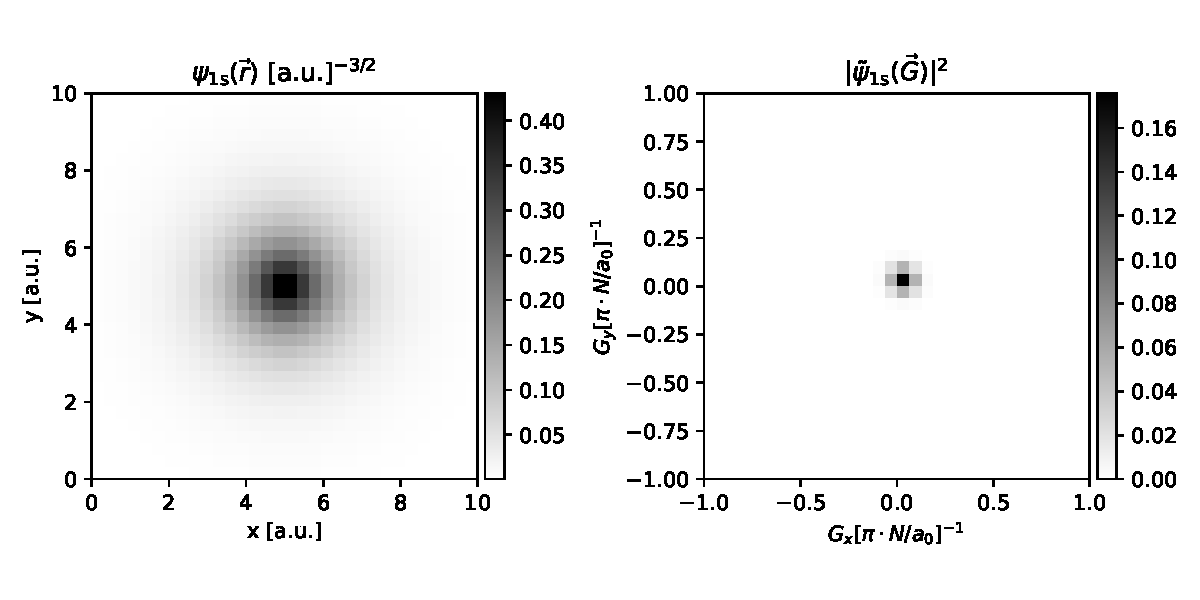
\includegraphics[width=\linewidth]{img/horb_1s_fields.pdf}
    \captionof{figure}{Scalar field of the 1s atomic orbital of hydrogen and its representation in reciprocal-space. The scalar and reciprocal field representations are shown at $z=5$ and $G_{z}=0$, respectively.}
    \label{fig:horb_1s_field}
\end{Figure}

From the right graph in \cref{fig:horb_1s_field} it can be readily seen that with increasing $\vec{G}$ magnitude, i.e. distance from the origin, the value of the expansion coefficient decreases.

The wave function as defined by \cref{eq:horb_1s} has an analytical solution for its kinetic energy, which can be readily found by solving\footnote{Spherical coordinates are used here. Note that the $4\pi$ term corresponds to the integration over the azimuthal and polar angles. The $r^{2}$ corresponds to the radial part of the Jacobian in this coordinate system.}

\begin{align}
    E_{\text{kin}} &= \left<\psi_{\text{1s}} \left| -\frac{1}{2} \nabla^{2} \right| \psi_{\text{1s}}\right> \\
    &= 4 \int dr \; r^{2} \exp \left( -r \right) \cdot \left(r^{-2} \frac{d}{dr} \left( r^{2} \frac{d}{dr} \exp \left( -r \right)\right)\right) \\
    &= \frac{1}{2}. \label{eq:kinen}
\end{align}

In what follows, three metrics are being assessed as function of the number of sampling points per Cartesian direction, being

\begin{enumerate}
    \item The total electron density evaluated by numerical integration in real-space.
    \item The sum of squared plane wave expansion coefficients
    \item The kinetic energy
\end{enumerate}

The first two metrics should both result in a value of unity, the latter corresponds to the analytical solution of \cref{eq:kinen}. In \cref{fig:ekin_convergence}, the relative error for these three metrics is shown. From this Figure it can be seen that with increasing number of sampling points, the relative error for all three metrics consistently decays.

\begin{Figure}
    \centering
    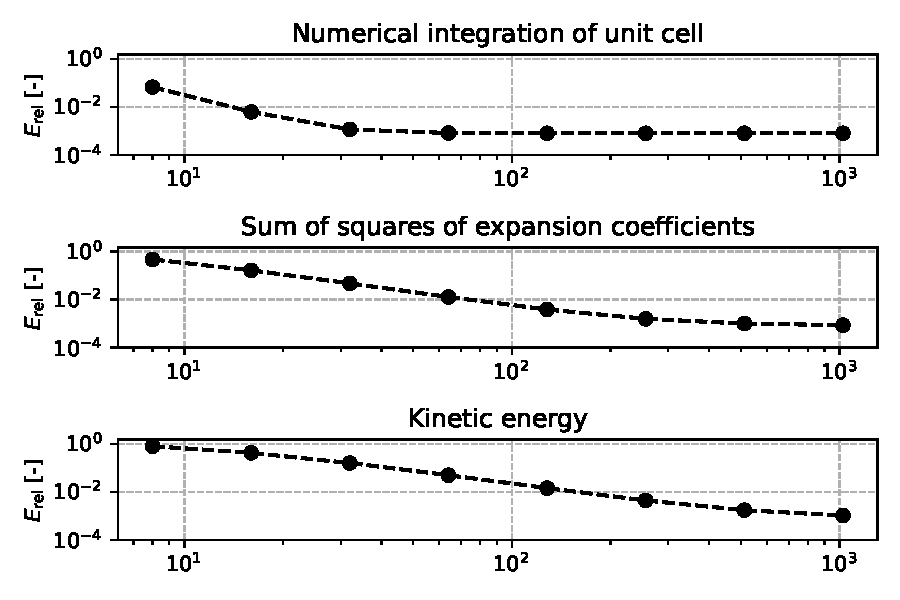
\includegraphics[width=\linewidth]{img/ekin_convergence.pdf}
    \captionof{figure}{Convergence of self-overlap and kinetic energy as function of the number of sampling points per Cartesian direction.}
    \label{fig:ekin_convergence}
\end{Figure}

Through both numerical and analytical approaches, key metrics such as the total electron density, the sum of squared plane wave expansion coefficients, and the kinetic energy are evaluated, showing that the numerical results converge to their expected values as the number of sampling points increases. The relative error in all three metrics systematically decreases with finer sampling, confirming the accuracy and reliability of the computational methods used in this analysis. As the number of sampling points relates to the number of planes waves, it follows that the cut-off energy, characterizing the number of plane waves in the basis set, is thus an easy parameter to use to set the accuracy and efficiency of the calculations.